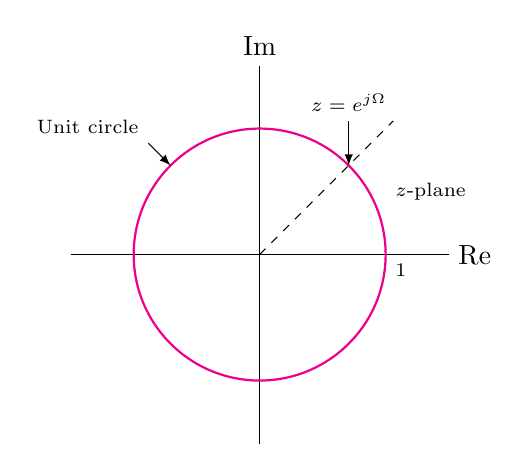
\begin{tikzpicture}[scale=0.8]
    \def\pole{++(135:0.1) -- ++(-45:0.2) ++(135:0.1) -- ++(45:0.1) -- ++(-135:0.2) +(45:0.1)}
    \def\zero{circle (0.1)}
    \draw (-3, 0) -- (3,0) node[anchor=west] {$\mathrm{Re}$};
    \draw (0, -3) -- (0,3) node[anchor=south] {$\mathrm{Im}$};
    \pause
    \draw[thick, magenta] (0,0) circle (2);
    \draw [latex-] (0,0) ++(135:2) -- ++(135:0.5) node [anchor=south east] {\scriptsize Unit circle};
    \node at (2, 0) [anchor=north west] {\scriptsize $1$};
   \pause
    \draw[dashed] (0,0)-- (45:3);
    \draw[latex-]  (0,0) ++(45:2) -- ++(90:0.7) node[anchor=south] {\scriptsize $z=e^{j\Omega}$};
    \node at (2, 1) [anchor=west] {\scriptsize $z$-plane};
\end{tikzpicture}